
\section{Das Lernmodul}\label{lernmodul}


\subsection{Grunds"atzliches}

\subsubsection{Die Philosophie}

Die zentralen Ans"atze:

\begin{list_sabina}
        \item 
	\textbf{Modularit"at des Lerninhaltes}:\\ 
	Lernmodule m"ussen strikt modular aufgebaut sein und aus den nachstehend
	beschriebenen Elementen und Subelementen \textit{vollst"andig} 
	zusammengesetzt werden k"onnen\footnote{Nur damit sind alternative, 
	benutzerspezifische Anordnungen m"oglich.}. 
        \item 
	\textbf{Visualisierung der Zusammenh"ange}:\\
	Ein Hauptanliegen (und auch der besondere Ansatz dieses Projektes) ist
	das Transparentmachen von mathematischen Zusammenh"angen.
        \item 
	\textbf{Erweiterbarkeit -- "Ubertragbarkeit}:\\ 
	Alle Strukturen m"ussen sich "uber Attributsysteme, Suchmaschinen
	und andere \textit{Automatismen} selbst"andig miteinander 
	verbinden\footnote{H"ort sich ehrgeizig an, ist es auch, ist aber unbedingt
	notwendig: Geschieht das nicht automatisiert, werden bei Erweiterung 
	bereits gezogenen Verbindungen falsch.}.
\end{list_sabina}

Zusammengenommen: \textit{kein} ``lineares Lehrbuch'', sondern ein
nichtlineares (vernetztes) wirklich multimediales Tool!



\subsection{Die inhaltliche Struktur}\label{inhaltliche_struktur_lernmodul}

\subsubsection{Die Hierarchie der Objekte}

\begin{list_sabina}
        \item \textbf{Kurs}: z.B. Lineare Algebra, Analysis, ...
        \item \textbf{Subkurs}: z.B. Differentiation und Integration, ...
        \item \textbf{Modul}: z.B. der Gau"salgorithmus, die Norm, 
        \item \textbf{Teilpfad}: ein m"oglicher Pfad innerhalb eines Modul (falls mehrere) 
        \item \textbf{Submodul}: ein Element mit all seinen abh"angigen Subelementen
        \item \textbf{Elemente}: z.B. Theorem, Definition, ...
        \item \textbf{Subelemente}: i.a. eindeutig zu einem Element geh"orende erg"anzende Inhalte
\end{list_sabina}



\subsubsection{Verf"ugbare Elemente und Subelemente}

Es gibt eine feste Anzahl an Elementen, die jeweils verschiedene
Subelemente haben k"onnen. Ein Subelement darf keine weiteren
Subelemente haben. Die Liste \textit{aller} verf"ugbaren Subelemente
wird in Kap. \ref{sub_elemente} beschrieben.


\paragraph{Die Elemente}\label{elemente}

\mbox{ }
\vspace{0mm}

    \begin{enumerate}
    \item Motivation
    \item Definition
    \item Theorem
    \item Algorithmus
    \item Anwendung
    \end{enumerate}


\paragraph{Die Subelemente}\label{sub_elemente}

\mbox{ }
\vspace{0mm}


    \begin{enumerate}
    \item Beweis
    \item Herleitung
    \item Bemerkung 
    \item Geschichte
    \item Motivation (zum Hauptelement)
    \item Visualisierung
    \item Beispiel
    \item Tabelle (im Sinne einer Liste)
    \end{enumerate}


\paragraph{Verkn"upfung von Elementen und Subelementen}\label{elemente_und_sub_elemente}

\mbox{ }
\vspace{0mm}

   \begin{enumerate}
    \item \textbf{Motivation (zum Modul)}\\
        verf"ugb. Subelemente: Historisches, Bem. \hfill{(unten links)}\\ 
	\phantom{verf"ugb. Subelemente: }Visualisierung, Bsp. \hfill{(unten rechts)}\\[-5mm]
	\begin{center}
	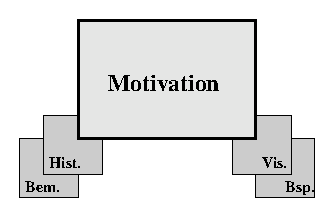
\epsfig{file=Skizzen/elemente_an_mot.eps, height = 2.8cm}
	\end{center}
    \item \textbf{Definition}\\
        verf"ugb. Subelemente: Mot. zu Def., Historisches, Bem. \hfill{(unten links)}\\
	\phantom{verf"ugb. Subelemente: }Visualisierung, Bsp., Tabelle \hfill{(unten rechts)}\\[-5mm]
	\begin{center}
	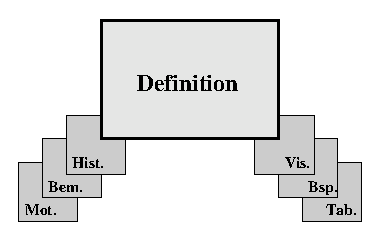
\epsfig{file=Skizzen/elemente_an_def.eps, height = 3.1cm}
	\end{center}
    \item \textbf{Theorem}\\
        verf"ugb. Subelemente: Herleitung \hfill{(oben links)}\\
	\phantom{verf"ugb. Subelemente: }Beweis \hfill{(oben rechts)}\\
	\phantom{verf"ugb. Subelemente: }Mot. zu Theorem, Historisches, Bem. \hfill{(unten links)}\\
        \phantom{verf"ugb. Subelemente: }Visualisierung, Bsp., Tabelle \hfill{(unten rechts)}\\[-5mm]
	\begin{center}
	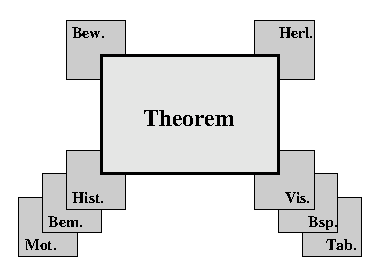
\epsfig{file=Skizzen/elemente_an_theorem.eps, height = 3.7cm}
	\end{center} 
    \item \textbf{Algorithmus}\\
        verf"ugb. Subelemente: Mot. zu Algo., Historisches, Bem. \hfill{(unten links)}\\
        \phantom{verf"ugb. Subelemente: }Visualisierung, Bsp. \hfill{(unten rechts)}\\[-5mm]
	\begin{center}
	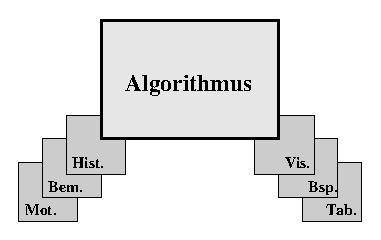
\epsfig{file=Skizzen/elemente_an_algo.eps, height = 3.1cm}
	\end{center} 
    \item \textbf{Anwendung}\\
        verf"ugb. Subelemente: Mot. zu Anw., Bem., Historisches \hfill{(unten links)}\\
        \phantom{verf"ugb. Subelemente: }Visualisierung, Bsp., Tabelle \hfill{(unten rechts)}\\[-5mm]
	\begin{center}
	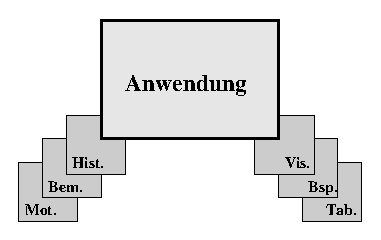
\epsfig{file=Skizzen/elemente_an_anwend.eps, height = 3.1cm}
	\end{center} 
    \end{enumerate}

Verf"ugt ein Element "uber mehrere Subelemente an derselben Position
(ein Satz etwa "uber Bsp., Visualisierung und Tabelle), so werden
diese Subelemente in immer derselben festen Reihenfolge angehangen:

\begin{list_sabina}
        \item 
	\textbf{unten links}: Mot. zu ... \textit{vor} Bem., \textit{vor} Historisches
        \item 
	\textbf{unten rechts}: Visualisierung \textit{vor} Bsp. \textit{vor} Tabelle
\end{list_sabina}

%(Oben links und rechts ist jeweils nur \textit{ein} m"ogliches
%Subelement vorgesehen: das Reihenfolgenproblem stellt sich hier somit
%nicht.)


Liegen mehrere Subelemente desselben Typs an einem Element vor, wird
nur \textit{ein} Symbol dort angehangen\footnote{Anderenfalls droht
bei Ausbau des Projekts eine ``graphische Katastrophe''...}


\subsubsection{Parallele und "aquivalente Pfade}

Parallele und "aquivalente Pfade sind wie folgt definiert:

\begin{list_sabina}
        \item 
	\textbf{parallele Pfade:}\\
	Parallele Pfade f"uhren mit \textbf{unterschiedlichen
	Herangehensweisen} zum gleichen Ziel. \\
	Bsp.: Der Gau"salgorithmus kann "uber elementare Zeilenumformungen
	\textit{oder} "uber Elementarmatrizen entwickelt werden. \\
	Charakteristisch f"ur parallele Pfade ist, da"s ein Lehrender
	beim Studium \textit{beider} Pfade tats"achlich \textit{mehr}
	(n"amlich unterschiedliche Zug"ange, verschiedenes Vokabular, ...)
	lernen w"urde als beim Studium nur eines.
        \item 
	\textbf{"aquivalente Pfade:}\\
	"Aquivalente Pfade f"uhren mit \textbf{unterschiedlichen
	Reihenfolgen} zum gleichen Ziel. \\
	Bsp.: Die Determinante kann "uber ihre Berechnungsvorschrift
	definiert werden, ihre Eigenschaften folgen dann als Satz;
	sie kann aber auch "uber ihre Eigenschaften definiert werden,
	die Berechnungsvorschrift folgt dann als Satz. \\
	Charakteristisch f"ur "aquivalente Pfade ist, da"s ein Lehrender
	beim Studium \textit{beider} Pfade \textit{nicht mehr} 
	lernen w"urde als beim Studium nur eines;
	die Reihenfolge ist mehr eine (didaktisch motivierte)
	``Geschmacksfrage''...
\end{list_sabina}

Aus der offensichtlich unterschiedlichen Relevanz dieser beiden
``nebeneinander'' existierenden Pfadtypen ergeben sich auch
unterschiedliche Darstellungen im Layout des Navigationsnetzes
(s. Kap. \ref{navigationsnetz}), 
kurz gesagt: parallele Pfade sollte man stets parallel sehen k"onnen,
"aquivalente nicht.


\subsection{Die Pr"asentation}

\subsubsection{Die Pr"asentation eines Kurses bzw. Subkurses}

Hier mu"s stehen, wie einem Benutzer eine "Ubersichtsanzeige ``seines''
Kurses (dessen Module und deren Abh"angigkeiten) pr"asentiert werden
kann.

Ausgehend von diesen geht er dann auf die Detaildarstellung der
einzelnen Module, sprich der Zusammensetzung der Module aus Elementen
und Subelementen, "uber. Dazu steht schon einiges im zugeh"origen
Kapitel.


\subsubsection{Die Pr"asentation eines Moduls bzw. Submoduls}

\paragraph{Das Hauptfenster}

\mbox{ }
\vspace{0mm}

Das Hauptfenster der Modul-Darstellung unterteilt sich in

\begin{list_sabina}
        \item \textbf{zentrale Men"uleiste} (f"ur globale Optionen)
        \item \textbf{Navigationsnetz} (f"ur die interaktive Pr"asentation des speziellen Moduls)
        \item \textbf{zentrales Inhaltsfenster} (f"ur den inhaltlichen ``Hauptinput'')
\end{list_sabina}

\begin{figure}[h]
\begin{center}
\input{Skizzen/hauptfenster_lernmodul.latex}
\caption{Layout des Hauptfensters}
\end{center}
\end{figure}

Auf Wunsch des Benutzers sollte das Navigationsnetz von dem restlichen
Fenster 'abgetrennt' werden k"onnen (Button auf zentraler
Men"uleiste).

\paragraph{Die zentrale Men"uleiste}\label{zentrale_menuleiste}

\mbox{ }
\vspace{0mm}

In der zentralen Men"uleiste werden untergebracht:

\begin{list_sabina}
        \item f"ur das Lerntool zentrale Men"upunkte
        \item f"ur das gesamte Projekt zentrale Men"upunkte
\end{list_sabina}

Es zerf"allt somit in (mindestens) zwei Bereiche.

%    Icon-Ideen: \\
%    rotes Wollkn"auel = roter Faden, Spinnennetz = Netz\\

Hier werden die f"ur das Lernmodul lokal ben"otigte Buttons, Optionen,
Icons gesammelt (in zwei Listen, s. S. \pageref{drei_bereiche_menuleiste}):

Men"upunkte, die grunds"atzlich im gesamten Projekt auftreten, aber in
Abh"angigkeit vom gerade gew"ahlten Tool des Projektes leicht
unterschiedliche Funktionsweisen besitzen:
        
\begin{list_sabina}
        \item \textbf{Bookmark}\\
        Seite (Element/Subelement) merken
        \item \textbf{Print}\\
	Drucken des aktuellen (Sub-)elementes;
	drucken des gesamten Modules (in Reihenfolge des 
	``roten Fadens'', ...
        \item \textbf{Help Lokal}\\
        soll verschiedene zus"atzliche\footnote{Einige Hilfefunktionen
	werden bereits in die (Sub-)Elemente direkt integriert} 
	lokale Hilfefunktionen anbieten
\end{list_sabina}

F"ur das jeweilige Tool des Projektes spezielle Men"upunkte

\begin{list_sabina}
        \item \textbf{Verbindung(en) zum "Ubungsmodul}\\
	bewirkt kein Verlassen des Lernmodules:
	zu allen Elementen und Subelementen des Moduls werden 
	die zugeh"origen (verschiedenen Typen von) "Ubungsaufgaben
	(s. Kap. \ref{uebungsaufgaben_typen})\footnote{Da (insbesondere
        in der Anfangsphase) \textit{nicht} "uberall "Ubungsaufgaben
	vorhanden sein werden, mu"s jeweils deutlich werden 
	(aktiver/inaktiver Button), ob 
	Aufgaben (zu den verschiedenen Typen) verf"ugbar sind.} 
	zug"anglich gemacht.
        \item \textbf{Forward/Backward}\\
        Durch Pfeile kann man im kanonischen Weg (d.h. roter Faden
        bzw. anderer sinnvoll definierter Weg, jeweils relativ zu der
        Position, an der man sich befindet,) vor- und
        zur"uckgehen. 
        \item \textbf{Multi/Single-Windows-Button}\\
        Wechselt zwischen der integrierten und der 
	Multi-Windows-Version (s. \ref{single_multi_windows}).
        \item \textbf{Trenn-Button}\\
        trennt das Navigationsnetz ab in eigenes Fenster
        \item \textbf{Modul-Pr"asentations-Button}\\
        wechselt von der ``normalen'' Ansicht auf den Pfad
	des vorliegenden Modules in zus"atzliche Sichten, 
	visualisiert weitere Umstrukturierung innerhalb eines Moduls
	(f"ur Neugierige und Profis). 
        \item \textbf{Hierarchie-Button}\\
        klettert in Modulhierarchie eine Stufe nach
        oben gelangen; Bsp: vom Modul zum Kurs (oder Subkurs?).
\end{list_sabina}


\paragraph{Das Navigationsnetz}\label{navigationsnetz}

\mbox{ }
\vspace{0mm}

In der Navigationliste wird das Netz des Moduls abgebildet. 

Die Elemente (siehe unten) werden durch ``K"astchen''\footnote{Das soll keine
Einschr"ankung an das sp"atere Layout sein, sondern nur eine Vorstellungshilfe...} 
dargestellt, in denen sich eine Abk"urzung und/oder ein Icon befindet, das
die Art des Elements angibt: Satz, Definition,...\\
Die Subelemente (siehe unten) werden in kleineren K"astchen leicht hinter die
Elemente geh"angt.\\
Dabei gelten die Anordnungsregeln aus Kap. \ref{elemente_und_sub_elemente}.

Die abgebildete Pfadstruktur ist bewu"st \emph{nicht linear}.\\
Der Studierende soll neben den reinen Inhalten auch deren
Zusammenh"ange und Abh"angigkeit visuell erleben k"onnen.

Der in Abh"angigkeit vom Benutzerprofil empfohlene Weg ist durch einen
``roten Faden'' \textbf{linear} (``Lern-Reihenfolge'', schlie"slich
ist Zeit linear) gekennzeichnet.\\ 
Der ``Forward/Backward-Button'' erm"oglicht die Bewegung entlang des
roten Fadens in einfacher Weise, 
auch k"onnen die K"astchen alternativ \textit{direkt} angeklickt werden
(damit stehen dem Benutzer immer auch andere Reihenfolge zur 
Verf"ugung).

Die Art des Elemente und Subelemente mu"s durch Farben, Icons oder
"ahnliches gekennzeichnet sein\footnote{F"ur Beschriftung sind
mindestens die Subelemente viel zu klein, die Elemente k"onnten
\textit{einen} Buchstaben tragen; diese Gr"o"senbeschr"ankung
entsteht, weil einerseits das Navigationsnetz keinesfalls durch
Scrollbars zerst"uckelt werden darf, andererseits aber ein gesamtes
Modul darstellen soll.}.

Mouse-Aktionen k"onnen weitere "Ubersichtsm"oglichkeiten schaffen:

\begin{list_sabina}
        \item \textbf{Mouse-over}\\
        Zoom-Effekt, Element mit seinen Subelementen erscheint
	vergr"o"sert und mit Mini-Abstrakt/Titel
        \item \textbf{Mouse-out}\\
        Zoom-Effekt verschwindet wieder
        \item \textbf{Left-Mouse-Click}\\
	Inhalt erscheint im zentralen Inhaltsfenster
        \item \textbf{Right-Mouse-Click}\\
	Inhalt erscheint, aber in Extrafenster (zum ``Festhalten'')
\end{list_sabina}

\marginpar{Farbskizze bringen wir mit}

Zus"atzlich k"onnten folgende Mouse-Bewegungen m"oglich sein:

\begin{list_sabina}
        \item \textbf{Mouse gegen oberen Rand schieben}\\
        Navigationsnetz des vorangegangenen Moduls erscheint 
        \item \textbf{Mouse gegen unteren Rand schieben}\\
        Navigationsnetz des nachfolgenden Moduls erscheint
        \item \textbf{Mouse gegen linken Rand schieben}\\
        Darstellung der "aquivalenten(!) Pfade (falls vorhanden) 
	wechselt:\\
	Default ist die ``"Ubereinanderdarstellung'',\\
	wechselt dann zur ``Paralleldarstellung''
\end{list_sabina}

\marginpar{Vergleichende Skizze bringen wir mit}


\paragraph{Zentrales Inhaltsfenster f"ur die Elemente/Subelemente}\label{zentrales_inhaltsfenster}

\mbox{ }
\vspace{0mm}

Im zentralen Inhaltsfenster stehen die Elemente und, soweit
platztechnisch m"oglich, auch deren Subelemente\footnote{\textit{Was}
platztechnisch m"oglich ist, h"angt nat"urlich von der Browsergr"o"se,
somit von der Aufl"osung des Monitors ab: modernen Default w"ahlen als
Default w"ahlen, ber"ucksichtigen, da"s Aufl"osungen immer besser und
Monitore immer gr"o"ser werden, automatische Anpassung erm"oglichen
(javascript, KDE-Tool).} .

Es werden zwei verschiedene Layout-Konzepte realisiert:\\
Bei beiden werden soweit ``konfliktfrei'' m"oglich (d.h. i.w. ohne Scrollbar)
die Inhalte der Elemente und Subelemente in einem gro"sen
Fenster belassen. 

\begin{list_sabina}\label{single_multi_windows}
	\item \emph{(integrierte Version)}\\\label{integrierte_windows}
	Subelemente, die zus"atzlich zu einem Element pr"asentiert werden 
	sollen (z.B. Satz und Beweis), erscheinen im zentrales Inhaltsfenster
	darunter oder daneben (getrennt scrollbar, eigener frame).\\
	Scrollbars, die aus Umfangsgr"unden entstehen, werden in Kauf 
	genommen.\\
	Ausnahme: Gr"o"sere Applets. Sie werden in einem eigenen sinnvoll
	positionierten Fenster ge"offnet (und sollten nie
	mit einem Scrollbar versehen sein).
	\item \emph{(Multi-Windows-Version)}\\\label{multi_windows}
	Elemente oder Subelemente, die nicht mehr in das gro"se Fenster
	``passen'' (d.h. einen Scrollbar erzwingen), erscheinen in einem
	neuen Fenster. Dieses mu"s dann sinnvoll positioniert werden
	(rechts daneben).
\end{list_sabina}

Beide Ansichten werden zur Verf"ugung gestellt.\\
Der Nutzer kann zwischen den beiden Darstellungsarten entscheiden.\\
Es kann jederzeit wieder zwischen den verschiedenen Modellen
gewechselt werden (Button auf zentraler Men"uleiste).


\paragraph{Zur Pr"asentation der Elemente}

\mbox{ }
\vspace{0mm}

Im folgenden werden Ideen und ``Eckdaten'' f"ur die Elemente, deren
inhaltliche Aspekte und ihr Zusammenspiel mit ihren Subelementen
gesammelt (Sammlung, wird laufend fortgeschrieben):

\begin{enumerate}
        \item \textbf{Motivation}\\
	beliebig, m"oglichst kreativ, ansprechend\\
	wenn m"oglich: Platz f"ur ein (historisches) Bild, das durch
	Anklicken zu ``Historisches'' f"uhrt
	\item \textbf{Definition}\\
	...
	\item \textbf{Satz}\\
	...
	\item \textbf{Algorithmus}\\
	auch in integrierter Version Beispiele in Extrafenster f"ur ``1:1-Blick''
 	\item \textbf{Anwendung}\\
	...
\end{enumerate}


\paragraph{Zur Pr"asentation der Subelemente}

\mbox{ }
\vspace{0mm}

Im folgenden werden Ideen und ``Eckdaten'' f"ur die Subelemente, deren
inhaltliche Aspekte und ihr Zusammenspiel mit ihren Elementen
gesammelt (Sammlung, wird laufend fortgeschrieben):


	\begin{enumerate}
	\item \textbf{Beweis}\\
	Ein Beweis erscheint, falls der Satz nicht zu lang ist,
	unter bzw. neben dem Satz (der im Fenster
	stehen bleibt). \\
	Sollte der Satz zu lang sein, so wird f"ur den Beweis ein
	neues Fenster ge"offnet.\\
	Ein Beweis sollte, falls er nicht zu kurz ist, dynamisch gestaltet werden:
	man sieht erst nur die grobe Struktur und kann dann durch Anklicken eines
	Unterpunktes die ausf"uhrliche Version desselben bekommen.
	Diese wird dann rechts aus dem Fenster herausgefahren.
	\item \textbf{Herleitung}\\
	Vergleichbar mit Beweis.\\
	Herleitungen stehen aber \textit{vor} dem Satz (in der integrierten 
	Version Scrollbar, in der Multi-Windows-Version in einem eigenen Fenster).
	\item \textbf{Bemerkung}\\	
	...
	\item \textbf{Geschichte}\\
	Die Geschichte sollte immer (auch) durch Anklicken
        eines (historischen) Bildes auf der Motivationsseite
        erreicht werden k"onnen.\\
	In der integrierten Version erscheint die Geschichte im Hauptfenster, 
	in der Multi-Windows-Version in einem eigenen Fenster.
	\item \textbf{Motivation (zum Hauptelement)}\\
	...
	\item \textbf{Visualisierung}\\
	Visualisierungen sollten niemals durch Scrollbar zerst"uckelt werden,	
	auch nicht in der integrierten Version: sie bekommen (wenn gro"s)
	automatisch immer ein eigenes Fenster. 
	\item \textbf{Beispiel}\\
	...
	\item \textbf{Tabelle (im Sinne einer Liste)}\\
	...
	\end{enumerate}


\subsection{Das logische Modell}

\subsubsection{Verkn"upfungen und Umordnungen}

Jedes Modul hat 
\begin{list_sabina}
        \item keinen Vorg"anger (``allererste Grundlagen-Module'')
        \item genau einen Vorg"anger
        \item verschiedene alternative Vorg"anger (``oder'')
        \item verschiedene notwendige Vorg"anger (``und'')
\end{list_sabina}


Jedes Element hat in seinem Modul 
\begin{list_sabina}
        \item keinen Vorg"anger (gilt i.a.f"ur die Motivation)
        \item genau einen Vorg"anger
        \item verschiedene alternative Vorg"anger (``oder'')
        \item verschiedene notwendige Vorg"anger (``und'')
\end{list_sabina}


Jedes Subelement 
\begin{list_sabina}
        \item ist an genau ein Element gebunden (Normalfall)
        \item darf sich an mehrere Elemente anh"angen (``und'')
        \item kann eine zus"atzliche Beziehung zu einem Element haben, 
	an das es aber nicht angehangen wird\footnote{Diese Abh"angigkeit 
	taucht z.B. bei Beweisen eines Satz auf, die sich auf eine 
	bestimmte von mehreren m"oglichen Vorg"angerdefinitionen   
	beziehen.}
\end{list_sabina}

Diese Informationen bilden das \textbf{logische Modell} vollst"andig
ab.\\ 
Sie reichen aber noch nicht zu einer didaktisch sinnvollen Skizze der
Gesamt-Zusammenh"ange aus\footnote{Z.B.: die Reihenfolge mehrerer
'gleichberechtigter' S"atze innerhalb eine Pfades liegt damit nicht
fest; sie alle nebeneinander zu visualisieren w"urde aber
un"ubersichtlich}.

\marginpar{An dieser Stelle wird gerade gedacht...}


%    {\textbf{\emph{Umstrukturierung innerhalb eines Moduls}}}\\
%    In einem Teilpfad gibt es keine Umordnungen. (z.B. wird die
%    Reihenfolge 'gleichgeordneter' S"atze festgelegt). Allerdings
%    gibt es in den meisten Modulen alternative Definitionen zu
%    demselben Begriff. Um im Modul dies nicht
%    vorzugeben, kann es je eine Version pro m"oglicher Definition
%    geben und unter Umst"anden noch eine weitere, in der die
%    verschiedenen Definitionen hintereinander gelegt sind. In
%    letzterem Modul gibt es dann einen zus"atzlichen Beweis
%    "uber die "Aquivalenz der Definitionen.\\
%    Diese Variationen k"onnen auch noch zu einem sp"ateren Zeitpunkt
%    eingebunden werden, sie haben also nicht die h"ochste
%    Priorit"at.\\
%    Bei 'Crash-Kurs'-Benutzern sollte keine Wechselm"oglichkeit
%    zwischen den Modulvariationen geboten werden. Bei den anderen
%    kann man durch
%    ein Icon in der Kopfleiste ein Fenster bekommen, in dem man
%    zwischen den verschiedenen Variationen wechseln kann.\\
%    Verwirklichung:\\
%    Die Elemente m"ussen mehrfach existieren, je nach ihrem
%    Kontext in der jeweiligen Variation. Eigentlich jedes Element
%    in einem Modul ist von der Umstrukturierung betroffen.\\



\subsection{Weiteres zu Styles, Positionierungen, ...}

\subsubsection{Eingebundene Bilder/Applets}
    Kleine Bilder k"onnen im Text umflossen werden. Sie werden
    an den 'richtigen' Ort gesetzt und zwar entweder an den rechten
    oder an den linken Rand des jeweiligen frames.\\
    Nicht von Text umflossenen Bilder werden alle zentriert!\\
    Bilder oder Applets, die zu gro"s sind, werden in einem neuen
    Fenster angezeigt. Sie sollten selbstsprechend sein.



\subsection{Globale Links, related Buttons etc.}\label{globaleLinks}

    Zu allen Begriffen, die unter Umst"anden unbekannt sind, gibt
    es die M"oglichkeit, durch Anklicken mit der rechten Maustaste
    ein Men"u mit den folgenden Unterpunkten zu bekommen :

\subsubsection{Das Men"u}

\begin{enumerate}
    \item Die Kurzhilfe
    Es gibt ein kleines Fenster, in dem der Begleiter die
    wichtigsten Zusammenh"ange oder die Definition erkl"art.
    Alles eher ungenau und umgangssprachlich.
    \item Links zu anderen Modulen
    Zu jedem Begriff erh"alt man eine Liste von Links zu Modulen,
    die diesen Begriff 'enthalten'. Man kann dann in das passende
    Modul springen, das den gesuchten Begriff definiert und
    erl"autert.
    Man kann u.U. die Variation des Moduls aussuchen
    (wenn man Profi ist), vgl. Umstrukturierung.
     \begin{enumerate}
            \item kanonischer Modulaufbau, z.B. "uber die
            Definition mit der Potenzreihe
            \item Variation 1: z.B. Definition "uber den
            Grenzwert
            \item Variation 2: z.B. Definition "uber die
            Differentialgleichungen
            \item Variation mit parallelen Definitionen
        \end{enumerate}
    Es entsteht ein neues Fenster, in dem von nun an immer die
    Linkverbindungen auftauchen.\\
    \item Browsen in allen Modulen\\
    Ideen:\\
    1)
    Der Studierende soll die Chance bekommen, zu einem Begriff, z.B.
    Stetigkeit, durch die gesamte Mathematik zu browsen und damit
    eng verkn"upfte Definitionen und Zusammenh"ange
    kennenzulernen.\\
       Jedes Element mu"s eintragen, f"ur welchen Begriff es
    ("ubergreifend) interessant sein k"onnte. (Eine Liste,
    vielleicht beliebig lang?)\\Dann kann
    automatisch das passende Modul bzw. die passende Lerneinheit
    gefunden werden und zusammen mit dem jeweiligen Element in
    das assoziative Netz eingetragen werden.
    In diesem Netz d"urfen alle Paare (Modul, Element) gemischt
    und unverbunden stehen - ein assoziatives Netz eben. \\
    Module oder andere Oberbegriffe k"onnen nicht angeklickt
    werden, nur Elemente.\\
    Wird ein Element in dem ass. Netz angew"ahlt, so wird
    automatisch ein Teil des umliegenden Netzes in dessen
    'Umgebung' generiert und im linken Teil des Browser-Fensters
    angezeigt. Dort kann man nun hineinklicken.\\
    BILD zu ass. Netz!!!!!!!!!!\\
    2) $\rightarrow$ Lexikonmodul...???...
\end{enumerate}

\subsubsection{Verwirklichung}
    Jeder Autor mu"s die nachschlagbaren Worte als mathematische
    Begriffe kennzeichnen, z.B. \verb?\mb{stetig}?. 
    Nur diese sind dann ``anklickbar'' (Layout: dezente Umsetzung 
    der ``Anklickbarkeit'' suchen, sonst optisch st"orend) \\
    Um die Menge der Links zu einem Begriff zu reduzieren, soll
    die 'Suchmaschine' folgenderma"sen arbeiten:\\
    1) Wenn der Begriff als Satz identifiziert werden kann (Satz von
    ...), so wird nur innerhalb der S"atze gesucht.\\
    2) Wenn der Begriff als Algorithmus identifiziert werden kann (Satz von
    ...), so wird nur innerhalb der Algorithmen gesucht.\\
    3) Ansonsten alles durchsuchen!?


\subsection{Benutzer ``Dozent''}

Der studentische Benutzer wurde im Kap. \ref{profil_allg_studi}
beschrieben, die Definition seines Benutzerprofiles ist universell
f"ur das gesamte Projekt.

Dozenten ben"otigen zum Ausbau und zum Aufbau ihrer Vorlesungen
zus"atzliche ``dozentenorientierte'' Werkzeuge:


\subsubsection{Dozenten-Suchmachine}


F"ur Dozenten, die lediglich erg"anzendes Material suchen, wird
``lediglich'' eine spezielle Suchmaschine ben"otigt, die die
Unter-Struktur der Module (die Typen der vorhandenen Elemente und
Subelemente, siehe S. \pageref{elemente}) transparent macht. \\
Die Suche verbindet dann die inhaltliche Abfrage (z.B. gib mir
``Stokes'') mit dem gew"unschten Elemententyp
(z.B. ``Visualisierungen'').\\ 
Multiple Abfragen sollten wiederum m"oglich sein (z.B. gib mir
``Stokes'' $+$ ``Gauss'' hinsichtlich ``Visualisierungen'' $+$
``Beispiele'').

Diese Anfrage bringt den Suchenden zun"achst auf ein eigenes
"Ubersichtsfenster (weil die Anfrage i.a. mehrere Treffer ergeben
wird, die sich nicht einmal alle im gleichen Modul befinden m"ussen,
also nicht gleichzeitig sichtbar gemacht werden k"onnen), in welchem
er dann die einzelnen Treffer nacheinander anklicken kann: der Inhalt
erscheint dann im Hauptfester (S. \pageref{fenster_namen}) in genau
derselben Weise, wie ein das Projekt selbst"andig benutzender Student
den Inhalt gesehen h"atte: links das Navigationsapplet
usw. (s. Kap. \ref{rrr}).

Damit wird dem Dozenten automatisch ein weiterf"uhrendes
``Herumst"obern'' in der gew"unschten Thematik erm"oglicht.


\subsubsection{Kurs-Creator}


Hier mu"s der sog. ``Creator'' beschrieben werden: h"angt bei mir an
der Wand und mu"s aus Zeitgr"unden sp"ater beschrieben
werden\marginpar{Skizze bringen wir mit}


\subsection{F"ur die Autoren}

\subsubsection{Autoren-Organisationstool}

Hier mu"s der organisatorische ``Overview'' beschrieben werden: es
beinhaltet eine "Ubersicht "uber die zu realisierenden Module, denen
geplanter Autor, Status (kein komplettes Controlling, sondern ``nur''
zentrale Infos, die M"oglichkeit, Erg"anzungen f"ur den Autor zu
hinterlassen...  h"angt auch bei mir an der Wand und mu"s aus
Zeitgr"unden sp"ater beschrieben werden\marginpar{Skizze bringen wir
mit}


%    {\textbf{\emph{Definieren der Voraussetzungen}}}\\
%    Jedes Element mu"s sich merken, auf welche S"atze und
%    Definitionen es zur"uckgreift (redundante Informationen
%    vermeiden!!!), und aus welchem Modul diese stammen:
%    Vor: (genaue Voraussetzungen: z.B. ausformulierter Satz von
%    Bolzano Weierstra"s (redundant?) | Modulname des Moduls,
%    in dem die Vor. steht| Elementname der Voraussetzung)\\
%    Warum so umst"andlich? Es k"onnte einen Begriff in
%    verschiedene Definitionen geben (deshalb die genaue Formulierung),
%    es k"onnte ein Begriff zu verschiedenen Modulen f"uhren
%    (z.B. Stetig), deshalb der Modulname, es kann je nach
%    Variation verschiedene Elemente zum gleichen Satz geben, daher
%    der Elementname.\\
%    Es sollte eine Trivialit"atsgrenze existieren, unter der
%    keine Voraussetzungen angegeben werden.\\
%    Die Voraussetzungen k"onnen entweder als Verweise auf andere
%    (existierende!) Module gestaltet werden oder aber als Verweise
%    auf S"atze, Definitionen,... aus B"uchern. Dazu mu"s es also
%    einen \emph{Kanon aus Referenzb"uchern} geben.\\



\subsection{Verbindungen zu anderen Modulen}

Auf der zentralen Men"uleiste ist ein "Ubergang zu allen anderen Teilen
des Projektes vorgesehen.

Es bleibt aber zu kl"aren, wie genau dieser "Ubergang im einzelnen 
\textit{in Abh"angigkeit von aktuellen Ausgangspunkt} zu regeln ist...
 
\subsubsection{Verbindung zum "Ubungsmodul}

...


\subsubsection{Verbindung zu...}

...













